\documentclass[9pt]{osa-supplemental-document}
\setboolean{shortarticle}{false}

\title{Variant Calling for Noisy Reads}
\author{} %leave this blank
%% DO NOT ADD AUTHOR INFORMATION HERE; IT WILL BE ADDED DURING PRODUCTION

\usepackage{amssymb}

\setboolean{displaycopyright}{false} %copyright statement should not display in the  supplementary document

\begin{document}

\maketitle


\section{High level Overview:}

We have different haplotype sequences reads/ fragments, and we wish to preprocess the reads to reduce the noise in the given fragments and pass it to haplotype assembly algorithm. 

The noise is generally a sequencing error which is randomly distributed over the fragments which flips the bit for some variant location in few of the fragments. However some sequencing are prone to systematic sequencing errors, and these are classified falsely as variants. 

For a true variant the allele in the fragment depends on the haplotype it is sampled from however for the false variant this is not the case, since the alleles are homozygous in both the haplotype sequences.

Our goal is to identify these false variants, but the problem is we do not know the original haplotype pairs. 


But with the given reads we should be able to extract these false variant locations, as for the reads having common variants would either contain the same bit if they are sampled from the same haplotype, or would be complement of each other if sampled from the different haplotype for all the variants except for the false variant, since it is independent of the haplotype.

To find the false variant we operate over the fragment pairs and try to calculate the similarity of the reads and then calculate the probablity whether or not the two reads are sampled from the same haplotype. 

\subsection{Problem Formulation}
Given a reference genome $Ref$, and a set of reads $R$ of an alternate Genome $G$ sampled of a different human decide whether or not the site $S_i$, corresponding to the $i_{th}$ site is a variant site, i.e. is different compared to the reference genome $Ref$.
\subsection{Inputs}
\begin{itemize}
    \item A reference genome $Ref$ of len $ref\_len$ from which the comparison needs to be made.
    \item A set of reads $R$ sampled from alternate genome $G$ of the same length, with start index $st$ and end of the index $en$, which is its position in the reference genome $Ref$.
    \item The error probability of each of the allele in each of the sample (For simplicity using $e$ as a constant, $0 < e < 1$). 
    
\end{itemize}

Each read is in the form 0 or 1, 0 if it matches to the reference genome and 1 if it matches to the alt genome.
The reference genome is an already sampled genome (assuming it has no errors for simplicity).

\subsection{Output}
\begin{itemize}
    \item Determine whether or not a site with index $i$, corresponding to the reference genome is a variant site.
    \item If it is a variant site, with what confidence can we say it is actually a variant site.
\end{itemize} 




\subsection{Given the read partition probablity of variant to False}

Lets consider a variant $V_i$, an alelle at position i, at position i either the variant can be false that is it is a homozygous with either (0/0) or (1/1) configuration in H1, H2, the probablity of this happening would be P($V_3 \in $ False Variant = P($V_i$ is 0/0 or 1/1).

\begin{equation*}
\begin{split}
P($V_i \in (00, 11)$  $| R1 \in H1$ and $R2 \in H2$ ) = 1/2 * ( $(1-e)^{num\_ones}$*$e^{num\_zeros}$ + $(1-e)^{num\_zeros}$*$e^{num\_ones}$)
\end{split}
\end{equation*}


Where $R1 + R2 = R$ and $R1 \cap R2$ is $\phi$. 

As we can see since this does not depend on the partition R1 and R2, this will remain the same regardless how we decide to cluster our fragments. 

\subsection{Given the read partition probablity of variant to True}

Now we calculate the probablity for it to be heterozygous, that is it can come from a (0,1) or (1, 0) configuration from H1, H2. 
If we are given a set of fragments R1 and R2 are coming from H1, H2, we know the value van either be 0/1 or 1/0 would be. 

Given $R1 \in H1$, $R2 \in H2$: 
\begin{multline*}
P($V_i \in (0/1)$  | R1, R2) = $(1-e)^{num\_zeros \in R1} * e^{num\_ones \in R1}$ * $(1-e)^{num\_ones \in R2} * e^{num\_zeros \in R2}$    
\end{multline*}
Similarly for 1/0 we would get:
\begin{multline*}
P($V_i \in (1/0)$  $|$ R1, R2) = $(1-e)^{num\_ones \in R1} * e^{num\_zeros \in R1}$ * $(1-e)^{num\_zeros \in R2} * e^{num\_ones \in R2}$
\end{multline*}
The probablity of being 0/1 and 1/0 configuration of h1, h2 are equal to 1/2. 
Hence the probablity of the site being heterozygous is 
\begin{multline*}
P($V_i \in (0/1$ or $1/0)$) = 1/2*P($V_i \in (1/0)$  $|$ R1, R2) + 1/2*P($V_i \in (0/1)$  | R1, R2).
\end{multline*}
Hence we can say the site is actually a variant with the above probablity given the partition R1 and R2. 

\subsection{Marginalize over all the possible configuarations of R1 and R2}

To calculate the probablity of the variant being a False Variant can be stated as:
\begin{equation*}
    \begin{split}
    % P($V_i \in F$)  = $\sum_{\forall_{R1, R2 pairs$}}$ P($V_i$ \in F |$ R1, R2)$ . P(R1, R2)
    
     P($V_i \in F$) = \sum_{\forall_{R1, R2 pairs} $P(V_i$ \in F |$ R1, R2$) . P(R1, R2)

    \end{split}
\end{equation*}

%  P($V_i \in F$) = $\sum_{\forall_{R1, R2 pairs}P($V_i$ \in F |$ R1, R2)$ . P(R1, R2)


We know how to calculate the P($V_{i} \in F |$ R1, R2), but currently we dont have all the possible combinations of (R1, R2). 


Given the read configuration we know there can only be a few configuration for the possible values of R1, R2 pairs, which have significant probablity. 

Our job is now reduced to computing the probablities for which P($R1 \in H1, R2 \in H2$), is not limiting to zero 0.

Now we need to find the value of probablity where fragments {$f1$, $f2$,... $fi,} \in R1$ and ($f3$, $f4$,.. $fj) \in R2$, such that R1 \cap R2 \in $\phi$. 

% \subsection{Estimate using the second order probablity distribution}


% There would be a total of $2^n$ different combinations of fragments selection from R1, R2, where n is the coverage for the given fragment. 

% However in the case of Haplotype assembly we can make inferences whether two of the fragments are sampled from the same haplotype with a good confidence.

% Since the sequencing error rate is low, if the fragments have a significant amount of match, we can with confidence say that it belongs to the same haplotype, and if for most parts one is the complement of each other then it is likely sampled from different haplotype.
% So we dont know what the actual haplotype is but we do know if two fragments are sampled from the same haplotype or not. 

% \begin{equation*}
% \begin{split}
%     P($f1$, $f2$,... $fi \in R1$, $f3$, $f4$,..$fj \in R2$) = P($f1$, $f2$,... $fi \in R1$)* P($f3$, $f4$,... $fj \in R2$)
% \end{split}
    
% \end{equation*}

% Given we can derive whether two fragments originate from the same haplotype, 
% we can estimate the above using a second degree approximation.

% \\
% \begin{multline*}
% P( ($f1$, $f2$,... $fi,) \in R1$ and ($f3$, $f4$,.. $fj) \in R2$) = \\
% P($f1 \in R1$)*P($f2 \in R1 | $ $f1 \in R1$)*P($fi \in R1 | $ $f_{i-1} \in R1$)*.....*\\
% P($f3 \in R2$)*P($f4 \in R2 | $ $f3 \in R2$)*P($fj \in R2 | $ $f_{j-1} \in R1$)
% \end{multline*}
% \\

% This can be said as a good approximation because of low sequencing error rate in general. 
% For example if we consider just three fragments: f1, f2, f3 (assuming it is sampled from the same fragment ) and if we dont take advantage of their structural property, the probablity of all the three coming from the same haplotype is  

% \begin{equation*}
% \begin{split}
%     P($f1, f2, f3 \in R1$) = $1/2^3$ 
% \end{split}    
% \end{equation*}
% \begin{equation*}
% \begin{split}
%     P($f1, f2, \in R1$, $f3 \in R2$) = $1/2^3$
% \end{split}    
% \end{equation*}

% And is the same for all the combinations of f1, f2, f3 coming from either R1 or R2, will have equal probablity. Hence the likelihood that f1, f2, f3 sampled from R1 would be the same as f1, f2, sampled from R1 and f3 sampled from R2. 

% However if we take advantage of the structural property, 
% we can calculate the probablity as:

% \begin{equation*}
% \begin{split}
%     P($f1, f2, f3 \in R1$) = P($f1\in R1$)*P($f2\in R1 | f1\in R1$) * P($f3\in R1 | f1, f2 \in R1$) 
% \end{split}    
% \end{equation*}

% \begin{equation*}
% \begin{split}
%     P($f1, f2 \in R1$, $f3 \in R2$) = P($f1\in R1$)*P($f2\in R1 | f1\in R1$) * P($f3\in R1 | f1, f2 \in R1$) 
% \end{split}    
% \end{equation*}

% Which can be simplified to a second order approximation:
% \begin{equation*}
% \begin{split}
%     P($f1, f2, f3 \in R1$) $\approx$ P($f1\in R1$)*P($f2\in R1 | f1\in R1$) * P($f3\in R1 | f2 \in R1$) 
% \end{split}    
% \end{equation*} 
% \begin{equation*}
% \begin{split}
%     P($f1, f2 \in R1$, $f3 \in R2$) $\approx$ P($f1\in R1$)*P($f2\in R1 | f1\in R1$) * P($f3\in R2 | f2 \in R1$) 
% \end{split}    
% \end{equation*} 

% How do we now find out P($fj \in R1 | $ $f_{j-1} \in R1$), that is both of the fragments belong to the same haplotype group.

% Given   $f_{j-1} \in R1$, we need to estimate the probablity $f_j \in R1$.

% If both the fragments are sampled from the same haplotype, we can say the intersection of both the fragments should be same, hence if it is same we have probablity of (1-e) and e if it is different. 

% \begin{equation*}
%     \begin{split}
%          P($f_j \in R1 | $ $f_{j-1} \in R1$) = $(1-e)^{matching\_bits}$*$e^{mismatching\_bits}$
%     \end{split}
% \end{equation*}

% And similarly if it belongs to the other haplotype group that is one is in set R1 while the other is in R2, would be the same with the powers e and (1-e) reversed. 
% \begin{equation*}
%     \begin{split}
%          P($f_j \in R1 | $ $f_{j-1} \in R2$) = $(e)^{matching\_bits}$*$(1-e)^{mismatching\_bits}$
%     \end{split}
% \end{equation*}


% If we divide the above we get 
% \begin{equation*}
%     \begin{split}
%          P($f_j \in R1 | $ $f_{j-1} \in R1$) / P($f_j \in R1 | $ $f_{j-1} \in R2$) = $((1-e)/e)^{matching\_bits}$*$(e/(1-e)^){mismatching\_bits}$
%     \end{split}
% \end{equation*}
% Rewriting:

% \begin{equation*}
%     \begin{split}
%          P($f_j \in R1 | $ $f_{j-1} \in R1$) / P($f_j \in R1 | $ $f_{j-1} \in R2$) = $((1-e)/e)^{matching\_bits - mismatching\_bits}$
%     \end{split}
% \end{equation*}

% We can see if the matching bits are greater than the mismatching bits the power becomes greater than one, and $(1-e/e) > 1$ since e is small, if we take e=0.05, $(1-e)/e \approx 20$.

% Hence for the example of f1, f2, f3 mentioned above:

% \begin{equation*}
% \begin{split}
%     P($f1, f2, f3 \in R1$) / P($P($f1, f2, f3 \in R1$)f1, f2 \in R1$, $f3 \in R2$) $\approx$ \\
%      P($f1\in R1$)*P($f2\in R1 | f1\in R1$) * P($f3\in R1 | f2 \in R1$) / \\
%     P($f1\in R1$)*P($f2\in R1 | f1\in R1$) * P($f3\in R2 | f2 \in R1$) 
% \end{split}    
% \end{equation*}

% \begin{equation*}
% \begin{split}
%     P($f1, f2, f3 \in R1$) / P($P($f1, f2, f3 \in R1$)f1, f2 \in R1$, $f3 \in R2$) $\approx$ \\
%      P($f3\in R1 | f2 \in R1$) /
%     P($f3\in R2 | f2 \in R1$) 
% \end{split}    
% \end{equation*}

% \begin{equation*}
% \begin{split}
%     P($f1, f2, f3 \in R1$) / P($P($f1, f2, f3 \in R1$)f1, f2 \in R1$, $f3 \in R2$) $\approx$ \\
%       $((1-e)/e)^{matching\_bits - mismatching\_bits}$
% \end{split}    
% \end{equation*}

% Hence we can see that if take advantage of the structural property we can calculate whether or not if the two fragments are sampled from the same haplotype, this can be estimated with a good confidence just by second order approximation. 

% That is if f2 and f3 have matching bits, its likelihood that all the the three being sampled from the same haplotype is much more that f1, f2 coming from one haplotype and f3 from other. 


\subsection{Estimating the likelihood of the variant coming from heterozygous genotype}

Now that we have established that the second order approximation of the fragments are a well enough measure for the likelihood measurement whether fragments are from the same pair or the different pairs. 
We come back to the original problem of calculating the probability of $i_{th}$
variant coming from a heterozygous genotype:
\\

\begin{equation*}
    \begin{split}
    % P($V_i \in F$)  = $\sum_{\forall_{R1, R2 pairs$}}$ P($V_i$ \in F |$ R1, R2)$ . P(R1, R2)
    
     P($V_i \in F$) = \sum_{\forall_{R1, R2 pairs} $P(V_i$ \in F |$ R1, R2$) . P(R1, R2)

    \end{split}
\end{equation*}

Given we know that we can estimate the likelihood pretty well just by knowing if another overlapping fragment is coming from the same sample.

Now we have N fragments, each fragment can either be sampled from either R1, or R2, and we can estimate its likelihood just by knowing the probability of the previous overlapping sample's probability of being sampled from either first or the second haplotype.
To find the likelihood of the given site to be heterozygous, we can continuosly update the value of the likelihood by updating the value of the likelihood given a fragment and using the information of previous fragments, and here we only need one fragment so the update step would look like: 

Hence for a variant, we iterate through all the fragments covering it, to get the likelihood of the variant originating from the heterozygous genotype.

Hence, we can simply write, the likelihood of fragment lying in R1 as:

\begin{equation*}
    \begin{split}
        L(i+1,  f_{i+1} $\in R1$) = L(i,  f_{i}  $ \in R1$)*P(f_{i+1} $\in R1 |$ f_{i} $\in R1$) + L(i,  f_{i}  $ \in R2$)*P(f_{i+1} $\in R1 |$ f_{i} $\in R2$)   
    \end{split}
\end{equation*}


and similarly for lying in R2 as :
\begin{equation*}
    \begin{split}
        L(i+1,  f_{i+1} $\in R2$) = L(i,  f_{i}  $ \in R2$)*P(f_{i+1} $\in R2 |$ f_{i} $\in R2$) + L(i,  f_{i}  $ \in R1$)*P(f_{i+1} $\in R2 |$ f_{i} $\in R1$)   
    \end{split}
\end{equation*}


Similarly we can iterate through all the fragments covering the site to calculate the likelihood values of the site being heterozygous given the last read is in R1, and also for the last read in R2.



if we know the $(i+1)_{th}$ fragment and the $i_th$ fragment have the same allele at site j, given and they both lie from the same haplotype, the probablity of this happening is (1-e), and if they have mismatching allele at site 

Given $i+1_{th}$ and $i_{th}$ are sampled from the same haplotype, the probability that the jth site is heterozygous,  \\

P( $G_j \in (0/1, 1/0) $ | $f_{i_{th}}, f_{i+1_{th}} \in R1$ ) = $(1-e)^{j_{th} bits are same}$ * $e^{j_{th} bits are different}$ \\

and similarly if $i+1_{th}$ and $i_{th}$ are sampled from the different haplotypes, the probability that the jth site is heterozygous,  \\

P( $G_j \in (0/1, 1/0) $ | $f_{i_{th}}$ \in R1, $f_{i+1_{th}} \in R2$ ) = $(1-e)^{j_{th} bits are different}$ * $e^{j_{th} bits are same}$\\

Hence we have the likelihood of the given site to be heterozygous as 
the sum of likelihood of both matching and mismatching value.

If the likelihood of this site, given the reads are low, we can tell with certain confidence that the site is homozygous, making it false variant.

\subsection{How do we order the fragments: Make a nearest neighbour graph}


Now the question arises for a given sets {f1, f2... f_{i}} $\in$ R1 and {f3, f4... f_{j}} $\in$ R2, how do we choose the pairs for the second order approximation of the joint probablity P({f1, f2... f_{i}} $\in$ R1 and {f3, f4... f_{j}} $\in$ R2)


\clearpage
\section{Genotype likelihoods without haplotype information}
Consider the set of reads $R$ covering a variant site V. We denote the two haplotypes by $H_1$ and $H_2$. We assume that each read is equally likely to be sampled from one of the two haplotypes. $e$ denotes the probability of sequencing error for each allele observed. Then, we can write:

\[ P(R|G) = \prod_r P(r|G) \]

where $G$ can take values 0/0, 1/1 and 0/1. For an individual read $r$ with allele '0':
\[ P(r=0|G=0/0) = \frac{1}{2}P(r|H_1,H_1[V]=0) +  \frac{1}{2}P(r|H_2,H_2[V]=0) = (1-e) \]


Similarly, for an individual read $r$ with allele '1':
\[ P(r=1|G=0/0) = \frac{1}{2}P(r|H_1,H_1[V]=0) +  \frac{1}{2}P(r|H_2,H_2[V]=0) = e \]

and

\[ P(r=1|G=1/1) = \frac{1}{2}P(r|H_1,H_1[V]=1) +  \frac{1}{2}P(r|H_2,H_2[V]=1) = (1-e) \]

\[ P(r=0|G=1/1) = \frac{1}{2}P(r|H_1,H_1[V]=1) +  \frac{1}{2}P(r|H_2,H_2[V]=1) = e \]



The interesting case is the for heterozygous genotype. For an individual read $r$ with allele '0':

\[ P(r=0 |G=0/1) = \frac{1}{2}P(r|H_1,H_1[V]=0) +  \frac{1}{2}P(r|H_2,H_2[V]=1) = \frac{1}{2} (1-e) + \frac{1}{2} e = \frac{1}{2} \]

and 

\[ P(r=1 |G=0/1) = \frac{1}{2}P(r|H_1,H_1[V]=0) +  \frac{1}{2}P(r|H_2,H_2[V]=1) = \frac{1}{2} e + \frac{1}{2} (1-e) = \frac{1}{2} \]

Therefore:

\[ P(R|G= 0/1) = \prod_r P(r|G=0/1) = {\frac{1}{2}}^n \]

\section{Genotype likelihoods with haplotype information}

Let $h(r)$ denote the haplotype of origin of read $r$ where $h(r)$ can take two values (1 or 2). 
Consider the case where we have two reads $r_1$ and $r_2$ that we know come from the same haplotype. The likelihoods for the homozygous genotypes $0/0$ and $1/1$ don't change. We can calculate the likelihoods $P(r_1,r_2|G=0/1, h(r_1) = h(r_2))$ as follows:

\[ P(r_1,r_2|G=0/1, h(r_1)=h(r_2)) = \frac{1}{2}P(r_1,r_2|G=0/1,h(r_1)=h(r_2)=1) +  \frac{1}{2}P(r_1,r_2|G=0/1,h(r_1)=h(r_2)= 2) \]

We have two cases for the alleles for reads $r_1$ and $r_2$:
\begin{itemize}
    \item $r_1 = 0, r_2=0$ or $r_1=1,r_2=1$:  $\frac{1}{2}{(1-e)}^2 + \frac{1}{2}e^2$
    \item  $r_1 = 0, r_2=1$ or $r_1=1,r_2=0$:  $e(1-e)$
\end{itemize}

The calculation shows that knowing whether two reads come from the same haplotype changes the likelihood for the heterozygous genotype. This likelihood calculation can be extended to all $n$ reads covering the variant site. Generalizing for $n$ reads coming from same haplotype given the site is heterozygous and the quality of each reads are the same, we get:

\begin{equation*}
%\begin{split}
P(r_1,r_2,\ldots r_n | G=0/1, h(r_1)=\ldots = h(r_n)) = \frac{1}{2}(1-e)^{n_0}*e^{n-n_0}   + \frac{1}{2}(1-e)^{n-n_0}*e^{n_0}
%\end{split}    
\end{equation*}

where $n_0 = \sum_i r_i$ and $e$ is the sequencing error rate.

Let $X = h(r_1),h(r_2),\ldots,h(r_n)$ denote the n-tuple corresponding to the haplotype of origin of the $n$ reads. Then, we can write: 

\[ 
p(R|G=0/1) = \sum_X p(R|G=0/1,X)p(X) 
\]


\subsection{Using second-order approximation for $p(x)$ to calculate likelihood}
Let us assume that the reads are ordered (to be determined) and the haplotype of origin of the $(i+1)$-th read depends only on read $i$. In other words, we can write: 

\[ p(X) = p(X_1) p(X_2|X_1) \ldots p(X_n|X_{n-1}) \]

Using this approximation, we can write

\[ 
 \sum_X p(R|G=0/1,X)p(X) = \sum_X p(r_1,r_2,\ldots,r_n|G=0/1,X_1,\ldots,X_n)p(X_1).p(X_2|X_1)\ldots p(X_n|X_{n-1})
\]

Rewriting,

\[
 \sum_{k=1,2} \left( p(r_1|G=0/1,X_1=k).p(X_1=k) \sum_{X[2..n]} p(r_2,\ldots,r_n|G=0/1,X_2,\ldots,X_n)p(X_2,\ldots,X_n|X_1=k) \right)
\]

%\[ \sum_{X[1..i-1]}p(r_1,r_2,\ldots,r_i|G=0/1,X_1,\ldots,X_{i-1}X_{i} = k)p(X_i=k) \]

Let $L_{ik}$ be the likelihood $p(r_1,r_2,\ldots,r_i|G=0/1,X_{i} = k)p(X_i=k)$ of the first $i$ reads calculated using the second-order approximation such that the $i$-th read is assigned to haplotype $H_k$. Note that this likelihood sums over all possible assignments for the first $i-1$ reads. Since the haplotype of origin of the $(i+1)$-th read only depends on $h(i)$, we can calculate $L_{i+1,k}$ using the following recursion: 

\[ L_{i+1,k} = L_{i,1} p(x_{i+1} = k | x_i = 1) p(r_{i+1}|G=0/1,x_{i+1} = k) + L_{i,2} p(x_{i+1} = k | x_i = 2)p(r_{i+1}|G=0/1,x_{i+1} = k) \] 

Base case:

\[ L_{1,1} = \frac{1}{2}e^{r_1}{(1-e)}^{1-r_1}\] and \[L_{1,2} = \frac{1}{2}e^{1-r_1}{(1-e)}^{r_1}\]
where we assume w.l.o.g that $H_1 = 0$ and $H_2=1$. 

\subsection{Ordering of reads}

Intuitively, the reads should be ordered such that consecutive reads overlap many heterozygous variants allowing us to calculate $p(X_i|X_{i-1})$ with high confidence. There are $n!$ possible orderings so we have to use some heuristic to find the "best" ordering.
Note that if we cannot calculate $p(X_i|X_{i-1})$ due to lack of overlap between the reads, then we can use $p(X_i|X_{i-1}) = p(X_i)$, i.e. the $i$-th read's haplotype assignment is independent of the previous read. 

\paragraph{Example:}
Suppose we have three reads $r_1, r_2$ and $r_3$ where $r_1$ covers variants $1$ to $5$, $r_2$ covers variants $6$ to $10$ and $r_3$ covers variants $1$ to $10$. In this case, if we know the haplotype assignment for read $r_3$, it determines the haplotype assignment for both $r_1$ and $r_2$ with high confidence. This example suggests that instead of an ordering, it may be better to think of a directed tree on the reads. However, we will have to modify the calculation in the previous section corresponding to the tree.....


\subsection{Calculating conditional probabilities}


\subsection{Algorithm for variant calling..}

If reads cover multiple heterozygous variants, we can compare the alleles at the overlapping heterozygous sites between a pair of reads to determine whether the reads come from the same haplotype or opposite haplotype. This requires knowing high-confidence heterozygous variant sites since only heterozygous sites can be used to differentiate between between the two haplotypes. 

Hence, haplotype information can be used to improve the accuracy of variant calling for heterozygous variants as follows:

%\paragraph{Variant calling algorithm:}
\begin{enumerate}
    \item calculate genotype likelihoods for each variant site without haplotype information and identify high-confidence heterozygous variant sites
    \item calculate genotype likelihoods for heterozygous sites using haplotype information 
    \item update the set of high-confidence heterozygous sites (i.e. remove sites for which the haplotype-based genotype likelihood is much worse than the standard genotype likelihood)
    \item repeat  steps 2 and 3 until convergence
\end{enumerate}







% \begin{equation*}
%     \begin{split}
%          P($f_j \in R2 | $ $f_{j-1} \in R1$) = $(1-e)^{matching\_bits}$*$e^{mismatching\_bits}$
%     \end{split}
% \end{equation*}






% \subsection{finding max $\alpha$}

% Since cohesiveness for a set is number of edges / num of vertices, 
% The cohesiveness of any set is of form $\beta$ / $n !$ where $\beta$ lies from 
% 0 to $n * n !$, hence we can binary search on $\apha$ to find the $\alpha$ such that the above algorithm returns True. 





% \subsection*{Proof of correctness}


% The graph H has a max\_flow, min-cut of finite value, hence we consider the cuts of finite capacity. 
% If there is a node of in cut A, such that its edge is in cut A`, we can safely say it is a not finite capacity cut, as there is a edge of infinite capacity going through it.

% Hence for  a cut to be of  a finite capacity the cut should be closed that is all the nodes and its corresponding edge's nodes should be in the same cut. 

% Now we find the value of the cut. 

% The value of the cut is 

% C (A, A`) = $\alpha  * \sum_{x_i \in A} count (x_i) $ + $\sum_{i,j \in A`} count(E i,j )$.

% Now if we add  and subtract  $\sum_{i,j \in A} count(E i,j )$.
% in the above term we get. 

% C (A, A`) = $\alpha  * \sum_{x_i \in A} count (x_i) $ - $\sum_{i,j \in A} count(E i,j )$ + $\sum_{i,j \in A`} count(E i,j )$ + $\sum_{i,j \in A} count(E i,j )$.

% We know $\sum_{i,j \in A`} count(E i,j )$ + $\sum_{i,j \in A} count(E i,j )$ is a constant K, as the number of edges are fixed for the given graph. 

% The above gets reduced to 

% C (A, A`) =   K - ( $\sum_{i,j \in A} count(E i,j )$ - $\alpha  * \sum_{x_i \in A} count (x_i) $)

% The value of $\alpha$ is nothing but the number of edges on number of nodes in the closed set S. 

% If the value $\alpha$ is feasible, the subtraction term would be 0. Hence if the cut is atleast K given value of $\alpha$ is feasible. 

% If the cut is atleast K for the given alpha, the min cut/ maxflow is also K for the given $\alpha$. 

% Hence if the max flow is K, the $\alpha$ is feasible. 


% Hence from the above we can say there is a set of cohesiveness $\alpha$ if the cut value is a


% Now we claim there is a set S with cohesiveness atleast $\alpha$ if 




% \subsection{Method to check if B1 can be nested in B2}
% \begin{algorithm}
% \caption{Greedy algorithm}\label{alg:euclid}
% \begin{algorithmic}[1]
% \Procedure{Can\_be\_nested}{$B1,B2$}\Comment(Check if B1 can be nested in B2)
% \State $B1\_dimensions$ = $sorted\_In\_Increasing\_Order(B1\_dimension)$
% \State $B2\_dimensions$ = $sorted\_In\_Increasing\_Order(B2\_dimension)$
% \State assert $length(B2\_dimensions)$ == $length(B2\_dimensions)$
% \For{$b1, b2$ in $B1\_dimensions, B2\_dimensions$} \Comment{check $b1 < b2$}
% \State If $b1 < b2:$ return False
% \EndFor\label{euclidendwhile}
% \State \textbf{return} $True$\Comment{Each dimension for b1 is less than b2}
% \EndProcedure
% \end{algorithmic}
% \end{algorithm}

% % We sort the dimensions of the Box $B_1$ and sort the dimensions of Box $B_2$, 
% % if each of the corresponding dimension of box $B_1$ fits into the dimension of Box $B2$, then and only then $B_1$ can be nested in $B_2$.

% \subsection*{Time Complexity}
% \subsection*{finding if $\alpha$ is feasible:}
% Time complexity can be number of O($N^3$) using Preflow push algorithm. 

% \subsection*{TO find max $\alpha$}
% To check we need to calculate whether the above algorithm return True for any $\alpha$ for $log(n.n!)$ times, i.e. $nlogn$ times.
% Time complexity O($n^4log(n)$)


% \section{Remote Sensors}

% High level Overview of the algorithm:

% We create a graph $H$ which has the sensors $s_i$ connected to super source $s$ with capacity $r_i$ and the base stations are connected to sink $t$ with capacity C. 
% The sensors are connected to each of the base stations that are within 2km of euclidean distance from the sensor with capacity $b_{i,j}$.

% We claim we have a possible solution iff we find a max flow of capacity $\sum_{\forall i \in n} r_{i}$ in the above network.

% \subsection{Proof of correctness:}

% Let $V = \sum_{\forall i \.in n} r_{i}$.

% If any of the sensors have bandwith less than $r_i$, then the max flow would be less than V, as we can find a min cut less than V when we cut the graph into s and $H - \{s\}$. As all the capacities have upper bound $r_i$, and atleast one of them is not fulfilled. 

% Hence for all the sensors to have $r_i$ bandwidth any cut of the graph should be atleast be equal to V.

% Similarly the  each base stations $B_i$ only supply to sensors which are within the range, with capacity $b_{i,j}$, and since the total supply is limited to C, at sink, the condition $\sum_{\forall{j}}b_{i,j}$  <= C is always satisfied.

% Hence when we get a max flow of V if all the conditions are satisfied. 

% We also need to prove if the we have all the conditions satisfied we would get a max flow of V. 

% If we have max flow of V lets assume, either of the conditions is not satisfied in hopes to contradict. 

% If any of the sensors bandwidth  is less than $r_i$, we can safely say that the 
% flow cannot be greater than V, as V can only be achieved if all the sensors are getting exactly $r_i$.

% Since the capacity of each base station $B_i$ is capped by C, and the connection between Base j and sensor i is also capped with $B_{i,j}$, we know if the max flow V is achieved all the conditions are being satisfied, as none of the paths can exceed the capacity. 

% Hence we know if we find the max flow to be $V = \sum_{\forall i \.in n} r_{i}$, we have a valid solution depicted by the flow else no possible solution. 


% \subsection*{Time Complexity:}
% The above graph has max capacity  $V = \sum_{\forall i \.in n} r_{i}$, and the number of edges as E $<$ (m+n + mn),  we can simply use Ford-fullerkson algo to get the answer in O(EV).
% Or we can use pre-flow push to calculate the max flow which has strict $O(N^3)$, where N is (m+n+2).

% % \subsection*{Proof of Correctness:}

% % We  have already proved that the nested relations are transitive relations in the above section. Hence in a graph if A points to B and B points to C, we know 
% % A can be nested in both B, and C and B can be nested in C.

% % Hence the len of the chain is the length of the nested sequence.
% % Now we know that the list of Boxes is sorted based on the their dimensions.

% % In hopes to contradict the assumption we say assume that we can find a better solution in the optimal solution which is greater than the solution from the algo. 

% % Consider the boxes from the algo as $( B_idx1, B_idx2, ....B_idxk)$ from solution which gives ans with len k-1, 

% % and we assume there is a different solution from optimal algorithm with length k. 
% % $( B_idy1, B_idy2, ....B_idyk, B_{idyk+1})$. 

% % Given the boxes are sorted in increasing order, for $B_idyi$ to nest in $B_{idyi+1}$, the box $B_{idyi+1}$ must lie in the sorted list after $B_idyi$.

% % Hence there should be a path from $B_idyi$ to $B_{idyi+1}$ in the graph constructed by our algorithm, as we proved that the relation is transitive.

% % Therefore there should be a path from $B_{idy1})$ to $B_idy2$ to $B_idy3$ to ... $B_{idyk+1})$ in the constructed graph.

% % Since there is a path with k+1 nodes, there path length is k, but we know the longest path length of the graph is k-1 as that is the final result of the solution. 
% % Hence from contradiction we can safely say that our algorithm does give the optimal solution.



% \section{Scheduling Medical Consulting}

% \subsection*{Condition A and B}
% Given the doctors are willing to work each day of given $L_i$, we make them work each day.
% Hence if for any day, the number of doctors willing to work on that day $q_i$ is less than $p_i$, we do not have a feasible solution. 
% Else the solution is simply picking up $p_i$ random doctors out of $q_i$. That would be our given list.

% If for any day i if $q_i < p_i$ there is no feasible solution, it means that means for some day i, the number of doctors willing to work on that day are less than $p_i$. 

% That means all doctors willing to work on that day are working and additionally we need to add some doctors who are not willing to work on day $p_i$. 


% \subsection*{Condition $A^*$ and $B$}
% If the previous algorithm returns the correct possible answer, that is our answer. If there is no such possible answer we build another graph G1. 
% Consider in the graph G above the max flow achieved $p1_i$ doctors for day i.
% We know 

% Create a graph G with 
%  - a doctor i as a node $doc_i$ connected to super source s with capacity c, 
 
%  - each day as a node $day_j$, connected with sink t with capacity $d_j = p_j - q_j$, where $p_j$ is the number of doctors needed on day j and $q_j$ are the number of doctors willing to work on day $j$. 
 
%  - Add edges between node corresponding to $doc_i$ and node $day_j$ where doctor i is does not have j in $L_i$, i.e. doctor i is not willing to work on day j.


% Let V $=$ $\sum_{i \forall i \in n} d_i$. 

% We claim if the flow of the above graph can be achieved as V, then we have a possible configuration defined by the flow of the above graph. 
% If we have a flow from $doc_i$ to $day_j$, we add $j$ to $L_i$.

% \subsection*{Proof of correctness}

% For 1. we make all the doctors work on all the days specified by them as there is no limit to the days.
% Hence for any day we have all the doctors willing to work on that day, if the number of doctors are greater, simply remove $p_i - q_i$ doctors randomly. 

% This would satisfy all the conditions A and B.

% If there is a day where $q_i < p_i$, that would mean all the doctors willing to work are working and still the capacity is yet to be filled. This means some doctors who are not willing to work need to be present on that day. 

% Hence the capacity for each day in the new graph is $max(p_i - q_i, 0)$.

% If we have the max flow V, we need to prove all the conditions satisfy. 

% In the graph each day can only atmost $d_i$ capacity, if any of the day has less capacity than $d_i$, we can say the flow is not V as ,
% V $=$ $\sum_{i \forall i \in n} d_i$. 
% Hence all the days now have $p_i$ doctors.

% Since the capacity between source and $doc_i$ is atmost c, there can be no flow greater than c, hence condition A is also satisfied.

% If all the conditions satisfy we need to prove max flow is V.

% If all the days have $d_i$ capacity in the $day_i$ to sink t node, we know the condition B, satisfyies. 
% Since all the capacities are limited to c , we know each doctor only works for atmost c days when he does not want to work. Condition A is satified.

% If all the capacities are saturated, the total flow is the sum of capacities, hence the total flow is V. 

% Hence when all the conditions are satisfied V is the max flow and when V is the max flow all the conditions are satisfied.


% Hence proved the correctness of the algo.





% % We need to minimize the rooms with condition that one class fits into the room, and no room can have two classes simultaneously scheduled.
% % There for is the size of class $C_i$ $<$ $R_j$ then class $C_i$ can be organized in room $R_j$, and no other class can use the room $R_j$. 

% % \subsection{Min number of Rooms used}
% % \begin{algorithm}[H]
% % \caption{Greedy algorithm}\label{alg:euclid}
% % \begin{algorithmic}[1]
% % \Procedure{Min\_number\_classes}{$B1,B2$}\Comment(Check if B1 can be nested in B2)
% % \State $C\_list$ = $sorted\_In\_Decreasing\_Order(C\_list)$
% % \State $R\_list$ = $sorted\_In\_Decreasing\_Order(R\_list)$
% % \state $room\_idx$, $class\_idx$ $=$ $0$, $0$
% % \State assert $len(R\_list)$ $>=$ $len(C\_list)$ \comment{other wise there are less rooms than classes}
% % \For{$r_i, c_i$ in $R\_list, C\_list$} \Comment{check $r_i > c_i$}
% % \State If $r_i < c_i:$ return False
% % \State Assign $r_i$ to class $c_i$
% % \EndFor

% % \State \textbf{return} $Assignments$
% % \EndProcedure
% % \end{algorithmic} 

% \subsection*{Time Complexity}
% For part A we simply assign all the doctors to all the days, making its time complexity O(MN).

% For the second we can use ford fullerkson with complexity O(C*E), 
% where E is (n*m) and C is V. 

% Or we can use preflow push which has complexity O($n^3$) where n is (num\_docs + num\_days).
% Complexity O($(num\_docs + num\_days)^3$).

% \section*{Cellular connections}
% Given we have G(V, E), we 
% Create a graph H where we have a node x representing each node of V and a node $y_{i,j}$ representing the edge between two nodes of V. 
% We connect the node $y_{i, j}$ to the source with capacity $b_{i,j}$ and similarly connect the site location x with the sink with capacity as $C_i$.
% And we connect the node $y_{i, j}$ to $x_i$ and $x_j$ with infinite capacity. 

% Claim: For the optimal solution the nodes of the sink side cut of the mincut represents the nodes to be constructed to get the maximum profit.

% The value of the optimal profit is nothing but the sum of all the profits for pairs i-j - the max\_flow of the given graph.

% \subsection*{Proof of correctness}

% The mincut of the graph is a finite site cut. 
% We know since the cut is finite sized cut edges with infinite capacity cannot pass through it.
% We initially chose the value of the all the edges to infinity for the edges that connect node i to any of its corresponding edges from G.

% Hence the nodes and its edges are a closed set, i.e. the nodes and its edges lie together in this set. 

% Hence the two node and edge sets are complementary. That is the edges in one side of the set do not have its nodes in the other cut set. 


% Note for a cut, the nodes i, j for any edge i,j will remain in the same cut, else the cut would not be of finite capacity, as the value of the edge between node i, edge i,j is infinite. 

% The value for cut for the given graph would be :
% C(A, A`) = $\sum_{i,j \in A} b_{i, j}$ + $\sum_{k \in A`} c_k$  

% If we add and subtract : $\sum_{i,j \in A`} b_{i, j}$ in the above term we get:
% C(A, A`) = $\sum_{i,j \in A} b_{i, j}$ + $\sum_{i,j \in A`} b_{i, j}$ + $\sum_{k \in A`} c_k$ - $\sum_{i,j \in A`} b_{i, j}$ 

% Hence 

% C(A, A`) = $\sum_{i,j \in A} b_{i, j}$ + $\sum_{i,j \in A`} b_{i, j}$ - ($\sum_{i,j \in A`} b_{i, j}$  -  $\sum_{k \in A`} c_k$  )


% We know   $\sum_{i,j \in A} b_{i, j}$ + $\sum_{i,j \in A`} $  = K (sum of all the possible profits to build all the sites),


% C(A, A`) = K - ($\sum_{i,j \in A`} b_{i, j}$  -  $\sum_{k \in A`} c_k$  )
% We know the value of  Profit(A`) = $\sum_{i,j \in A`} b_{i, j}$  -  $\sum_{k \in A`} c_k$ 

% If we minimize the value of the cut we can find the maximal profit of the set A`. 

% Hence the mincut would represent the set of locations for which the profit is maximized.

% Hence for the optimal solution the sink side cut represents the nodes to be constructed to get the maximum profit.  

% \subsection*{Time Complexity}
% We need to calculate the max flow min cut, We can use preflow push which has complexity O($n^3$) where n is (num\_edges + num\_vertices).
% Complexity O($(V+E)^3$).

% % \section{Business Plan}

% % High level description of Algo:

% % We want to optimize the profit for at most k jobs, and each job has positive profit and to start a job we need to have a initial amount X which should be greater than the initial amount that we have.

% % Base case for k = 1, for only 1 job we need to find the job which has initial cost $c$ which should be less than $C0$, and the profit should be maximized. 

% % Hence from all the pairs ($c_i, p_i$) where $c_i <= C_0$ , we choose the pair which has maximum $p_i$. 

% % Algorithm:

% % Pair all ($c_i, p_i$) for all the jobs and sort it.

% % 1 - Then search for all the jobs using binary search such that $c_i$ < $C$ $\forall$ $j \in (1, i)$ and consider this list as $L^`$.

% % 2 - Now perform a linear search on $L^`$ which has the maximum value of $p_j$, 
% % add the value of $p_j$ to $C$ and delete this element from the original list. 

% % Continue the same process (1, 2) for k iterations and get the final result $C$, making the final profit as $C - C_0$.

% % \subsection*{Algo Max profit}
% % \begin{algorithm}[H]
% % \caption{Greedy algorithm}\label{alg:euclid}
% % \begin{algorithmic}[1]
% % \Procedure{Max\_profit}{$C_0, C\_P\_list$}
% % \State $C$ = $C_0$
% % \State $C\_P\_list$ = $sorted\_In\_Increasing\_Order(C\_P\_list)$
% % \For{$i$ in $range(k)$} \Comment{Do it for all the k jobs}
% % \State Find the maximum index $i$ such that $c_i < C$ \Comment{Do this using Binary Search}
% % \State Find index $j$ such that $p_j > p_k \forall k \in (1, i)$ $\&$ $j < i$
% % \State C $=$ $ C + p_j$
% % \State delete $C\_P\_list[j]$
% % \EndFor
% % \State \textbf{return} $C$ - $C_0$   \Comment{return the maximum Profit}
% % \EndProcedure
% % \end{algorithmic}
% % \end{algorithm}

% % \subsection*{Time Complexity}
% % Initially we perform a sort on the list of pairs $(c_i, p_i)$ which takes $ON(Log(N))$
% % We perform $k$ iterations for each job, in each iteration we perform a binary search on the cost $c_i$ such that $i$ is maximum and $c_i$ < $C$. This takes $O(N(logN))$, where N is the number of jobs, and then we do a linear search to find the maximum index $j$ where $p_j$ is the max of all profits. This takes $O(N)$ time, hence the total time complexity for the loops are $O(k*(NlogN + N)$.
% % Hence the time complexity is $O(k*(NlogN)$.


% % \subsection*{Proof Of correctness:}

% % Base case: If we have $k$ = 1, then we need to find a job such that $c_i$ < $C$ and $p_j$ is maximum $\forall j \in (1, i)$. 
% % Given we have a sorted list and we perform a binary search, hence we get all the jobs satisfying $c_i$ < $C$.
% % And we find the maximum value of $p_j \forall j \in (1,i)$, hence we can safely say that this is the optimal answer. 

% % Assume we get the optimal answer using the above algorithm till index i. 
% % We know from the algorithm we have deleted all the jobs which have been previously selected,  hence we get the similar substructure where we have an initial price $C$ and set of jobs to choose from and k-i jobs left to choose. 

% % For index i+1 we need to prove that we are choosing the optimal job which maximizes the profit. 

% % In each iteration we see that we are performing a search to get all the possible values for index i, such that $c_i$ < $C$, hence we cannot choose any other job from outside this list since it wont satisfy the constraints. 
% % And if we choose some other value than the one chosen from algo we can prove that it is not optimal as the algorithm chooses $p_j$ where $p_j > p_x \forall x \in (1, i)$. Hence our algorithm chooses the optimal value of the job to maximize the profit. 
% % Hence our algorithm is correct.

% % \section{Shortest Wireless Path Sequence}

% % \subsection*{1:}
% % Given there is a common path $s-t$ sequence in all of the graphs $(G_0, G_1, .. G_b)$, we need to find shortest such path. 

% % Since we know that the s-t path ,it is possible to choose a single path P that is an s-t path in each of the graphs  $(G_0, G_1, .. G_b)$.
% % We need to find the shortest such path. Since we know the s-t paths are present in all of the graphs, that means it has the same common edges in all of the graphs. 
% % And we need to choose a path from the common edges of all the graphs, hence we
% % take an intersection of all the edges and say the edges after intersection is $E_{final}$.
% % And we perform a djikstras algorithm to find the shortest path from s-t. 
% % We know the djiskstra algorithm gives the correct answer for any graph with positive weights and since it is given that the weight is 1 for each edge, as it is given that the cost is the number of nodes travelled from s-t.

% % Since each path for adjacent nodes has weight 1, the priority queue changes to a queue has each path with weight 1, since it has each path with weight one the priority of each of the edge to be considered is the same. Hence it can be considered as a simple queue. 

% % Therefore the djikstras algorithm simply equals to the BFS algorithm in this case.
% % \\
% % \subsection*{Time Complexity}
% % To find the the common edges we need to perform a iterative intersection for each of the graph. 
% % We know there can be O($N^2$) number of nodes in each graph, 
% % and we need to check if each of the edge is present in graph $G_i$ $\forall$ i $\in$ $(1, B)$. 
% % Hence the time complexity to find the common edges in O($B*N^2$).
% % We know the time complexity to perform a BFS is O(N) where N is the number of nodes in the graph. 
% % Hence the total complexity turns out to be O($B*N^2$).
% % \\
% % \subsection*{Proof of Correctness}
% % Assuming the Djikstra algorithm gives the shortest path in a graph G with positive edge lengths.
% % we can safely say that the path we need to find must be common in all the graphs  $(G_0, G_1, .. G_b)$, else the path will not satisfy the given condition. 

% % Since we find the a graph $G^`$ which has all the common paths we can say that the shortest s-t path of $G^`$ is the shortest possible path of all the commong edges. 
% % And we know the djikstras algorithm gives the shortest path of a graph with positive weights, it is safe to say we are providing the correct algorithm. 

% % \subsection*{2: Minimize cost function}
% % Given we have a set of graphs $(G_0, G_1, .. G_b)$., we need to find a sequence of paths $p_0, p_1, p_2..p_b$ such that the cost function is minimized.  
% % Each path $p_i$ may or may not be same as the $p_{i-1}$.
% % If the path is not same as previous path we add a penalty of $K$ to the cost, else we simply add the length of the path $p_i$ to the cost function.

% % High level algorithm to minimize the cost:
 
% %  Consider a graph $G^`(i, j)$ which contains all the common edges for graphs
% %  $(G_i, G_{i+1}, .. G_j)$, and we denote the shortest path on this graph as 
% %  $P(i, j)$. This path $P(i, j)$ can be found using the above algorithm.
 
% % \subsection*{Algo Min cost}
% % \begin{algorithm}[H]
% % \caption{Dynamic Programming algorithm}\label{alg:euclid}
% % \begin{algorithmic}[1]
% % \Procedure{Min\_cost}{$(G_0, G_1, .. G_b)$}
% % \State $Cost$ = $S_0$ \Comment{The shortest path in $G_0$}

% % \For{$i$ in $range(1, B)$} \Comment{}
% % \State $cost_i$ = get\_shortest\_path($G^`_{0,i}$)
% % \For j in (2, i):
% % \State $Cost[i]$ = min($cost_j$, get\_shortest\_path($G^`_{j, i}$)*(i-j) + K)
% % \EndFor
% % \EndFor
% % \State \textbf{return} $Cost[B]$   \Comment{return the minimum cost}
% % \EndProcedure
% % \end{algorithmic}
% % \end{algorithm}


% % Base case: If we have a b = 1, that is we only have one just one graph to find the s-t path, and since there is just one path, we dont need to add a penalty,
% % so we only need to minimize the path length from s-t. Hence the answer is $S_0$.

% % Now we find the optimal cost till i and store in $Cost[i]$, now we move to the next graph G$[i+1]$, 
% % here we can choose a new path, which is common for graphs $(G_j, G_{j+1}, .. G_{i+1})$ $\forall j \in (2, i)$.

% % choose to have the same path used in $G_{i-1}$ if the path exists so that the penalty incurred for change of path is 0.
% % Or we could add a new path for $G_{i+1}$ with penalty incurred

% % Recursive Formulation:

% % Cost[i] = $P^`{(0, i)}$*(i) if there exists a common path in $G^`(0, i)$ 

% % Cost[i] = min(Cost[i],  Cost[j] + $P^`{(j, i)}$*(i-j) + K) 

% % where we change the path at $G_j$ where $j \in (2, i-1)$  and we incur penalty due to the change in path at $G_j$.

% % \subsection*{Time Complexity:}

% % In each iteration for i from (1, B), we find the shortest path in
% % get\_shortest\_path($G^`_{j, i}$)  $\forall j \in (1, i)$. 
% % Finding the shortest path in ($G^`_{j, i}$) takes time complexity $O(N)$, where N is the number of nodes, and we do this $\forall j \in (1, i)$ hence each loop has time complexity $O(N^2)$, and we do this for B steps, making the time complexity of the algorithm $O(B*N^2)$.

% % \subsection{Proof of Correctness:}
% % Proof using Induction.
% % Base case:
% % If we have a b = 1, that is we only have one just one graph to find the s-t path, and since there is just one path, we dont need to add a penalty,
% % so we only need to minimize the path length from s-t. Hence the answer is $S_0$.

% % We already prooved the base case correctness in the previous section. 

% % Now consider the algorithm gives the correct answer $\forall j \in (1, i)$. 

% % For i+1, we assume that there is a better answer than the one algorithm provides, and consider it as $C^`$, there are only two possibility that there never incurred a penalty to change the path, or the path did change at some indexes $(G_{idx1}, G_{idx2}, .. G_{idxk})$, which gives the optimal answer, with $idx1, idx2, ... idxk$ in increasing order and $idxk < i$

% % Since the algorithm gives the optimal answer till $idxk$, 
% % the optimal answer 

% % $C^`$ = min( C(idxk) + $P^`(idxk+1, i)$*(i-idxk+1)  + K,  $P^`(0, i)$*i )

% % As we can see in the algo, we iterate through all the values of j from (2, i). 
% % Since idxk lies in (2, i), our algorithm gives as good answer as the optimal algorithm.
% % Hence our algorithm is optimal .





% % \section*{5. Untangling Signal Superposition}

% % We need to find the some combination of $s1$ and $s2$ such that their combination in any order forms string $S$.

% % Since we can add multiple number of s1 strings and s2 strings, we create a string S1 which is a concatenation of s1 such that len(S1) >= len(S), and similarly for string s2 we create S2. 

% % Therefore if there is a combination of s1 and s2 in S, we can safely say the same combination lies in S1 and S2 respectively. 
% % Hence, we can say S is a combination of subsequence of S1, and S2. 
 
% % The problem is now to find a subsequence of S1 and S2 such that it forms S. 

% % Algo Dynamic Programming:

% % Concatenate $S1$ = $s1* k1$  such that len(S1) >= len(S), similarly 
% % Concatenate $S2$ = $s2* k2$ such that len(S2) >= len(S). 

% % Now the problem reduces to find whether some part of S1 and some part of S2 arranged in increasing order can together make S.

% % Subproblem:


% % We find iterate through all the combination of (i, j) from i and j ranging in Len(S). And check if the some combination of first i chars of S1, and some combination of first j chars of S2  can form S[i+j].

% % Consider: dp($i, j$) is True , if there exists a combination of (S1[i], S2[j])
% % which forms S[i+j]. 

% % Base case: dp(0,0) = True i.e., we take 0 len of S1 and 0 len of S2 which is equal to 0 len of S. 

% % \subsection*{Is tangled of S1, S2}
% % \begin{algorithm}[H]
% % \caption{Dynamic Programming algorithm}\label{alg:euclid}
% % \begin{algorithmic}[1]
% % \Procedure{Is\_tangles}{$(S1, S2, S)$}
% % \State dp(0, 0) = True
% % \For{$i$ in $range(1, len(S))$} \Comment{}
% % \For $j$ in range($1, len(S)$)
% % \State If (dp[i-1, j] and S[i+j] == S1[i]): dp(i, j) = True
% % \State If (dp[i, j -1] and S[i+j] == S2[j]): dp(i, j) = True
% % \EndFor
% % \EndFor
% % \For{$i$ in $range(1, len(S))$} \Comment{}
% % \For $j$ in range($1, len(S)$)
% % \State If (i+j = len(S) and dp(i, j) == True): return True
% % \EndFor
% % \EndFor
% % \State \textbf{return} False   \Comment{return the minimum cost}
% % \EndProcedure
% % \end{algorithmic}
% % \end{algorithm}

% % The answer is True given there exists a pair(i, j) such that i+j == len(S) and  dp[(i, j)] = True.
% % The last char of S[i+j] can either come from S1[i] or S2[j]. 

% % Recursive formulation:
% % dp(i, j) = True if we have dp(i, j-1) True and S2[j] == S[i+j]
% % dp(i, j) = True if we have dp(i, j-1) True and S2[j] == S[i+j]

% % \subsection*{Time Complexity:}

% % We find iterate through all the combination of (i, j) from i and j ranging in Len(S). And check if the some combination of first i chars of S1, and some combination of first j chars of S2  can form S[i+j]. 
% % Time complexity is O($N^2$).

% % \subsection*{Proof Of correctness}
% % Proof By Induction:


% % Base case: dp(0,0) = True i.e., we take 0 len of S1 and 0 len of S2 which is equal to 0 len of S, as empty string is equal to sum of two empty strings we can say the algo runs fine for base case. 

% % Consider for len(k) the algorithm gives the correct answer that is there exists a pair (i1, j1) whiere i1+j1 == k1, 

% % and it is formed using i1 len of S1 and j1 len of string S2.



% % For k = k+1, the value of string S[k+1] must be either a part of s1 or s2.
% % From algorithm we can see it is we only set it to True if either of the 

% % we have dp(i, j-1) True and S2[j] == S[i+j] or we have dp(i, j-1) True and S2[j] == S[i+j]. 
% % Hence we can see each step we take only part of S1 or S2 to make S. 
% % This satisfyies all the conditions specified in the problem, else we do not set it to True. 

% % This makes the k th step give the right answer. 
% % Hence from the above induction we know the algorithm gives the correct answer of any value of l. 

% % Hence the algorithm is correct. 




















% % \section{Numbering Items in the Supplementary Document}

% % The supplementary materials document may contain additional figures, tables, equations, etc. Such items should be numbered, with an uppercase “S” to identify them as supplementary. For example, number the first figure in the supplementary document “Fig. S1”; the first table “Table S1”; etc.

% % This template has been designed to automatically format these components with this styling, but we include the naming convention here for reference.

% % \subsection*{Naming Convention for Countable Items}

% % \begin{condenseditemize}
% % \item[] Algorithm S1
% % \item[] Equation (S1)
% % \item[] Figure S1
% % \item[] Media S1
% % \item[] Table S1
% % \end{condenseditemize}


% % \section{Figures and Tables}
% % Figures and Tables should be labeled and referenced in the standard way using the \verb|\label{}| and \verb|\ref{}| commands.

% % \subsection{Sample Figure}

% % Figure \ref{fig:false-color} shows an example figure.

% % \begin{figure}[htbp]
% % \centering
% % \fbox{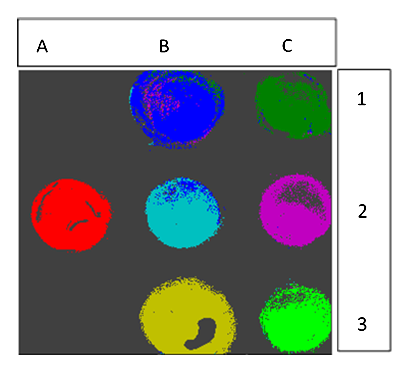
\includegraphics[width=.6\linewidth]{sample}}
% % \caption{False-color image, where each pixel is assigned to one of seven reference spectra.}
% % \label{fig:false-color}
% % \end{figure}

% % \subsection{Sample Table}

% % Table \ref{tab:shape-functions} shows an example table. 

% % \begin{table}[htbp]
% % \centering
% % \caption{\bf Shape Functions for Quadratic Line Elements}
% % \begin{tabular}{ccc}
% % \hline
% % local node & $\{N\}_m$ & $\{\Phi_i\}_m$ $(i=x,y,z)$ \\
% % \hline
% % $m = 1$ & $L_1(2L_1-1)$ & $\Phi_{i1}$ \\
% % $m = 2$ & $L_2(2L_2-1)$ & $\Phi_{i2}$ \\
% % $m = 3$ & $L_3=4L_1L_2$ & $\Phi_{i3}$ \\
% % \hline
% % \end{tabular}
% %   \label{tab:shape-functions}
% % \end{table}

% % \section{Sample Equation}

% % Let $X_1, X_2, \ldots, X_n$ be a sequence of independent and identically distributed random variables with $\text{E}[X_i] = \mu$ and $\text{Var}[X_i] = \sigma^2 < \infty$, and let
% % \begin{equation}
% % S_n = \frac{X_1 + X_2 + \cdots + X_n}{n}
% %       = \frac{1}{n}\sum_{i}^{n} X_i
% % \label{eq:refname1}
% % \end{equation}
% % denote their mean. Then as $n$ approaches infinity, the random variables $\sqrt{n}(S_n - \mu)$ converge in distribution to a normal $\mathcal{N}(0, \sigma^2)$.

% % \section{Sample Algorithm}

% % Algorithms can be included using the commands as shown in algorithm \ref{alg:euclid}.

% % \begin{algorithm}
% % \caption{Euclid’s algorithm}\label{alg:euclid}
% % \begin{algorithmic}[1]
% % \Procedure{Euclid}{$a,b$}\Comment{The g.c.d. of a and b}
% % \State $r\gets a\bmod b$
% % \While{$r\not=0$}\Comment{We have the answer if r is 0}
% % \State $a\gets b$
% % \State $b\gets r$
% % \State $r\gets a\bmod b$
% % \EndWhile\label{euclidendwhile}
% % \State \textbf{return} $b$\Comment{The gcd is b}
% % \EndProcedure
% % \end{algorithmic}
% % \end{algorithm}

% % \section*{Media}

% % The supplemental document may contain linked objects such as video, 2D, 3D, and machine-readable data files. Please see the \href{https://www.osapublishing.org/submit/style/supplementary_materials.cfm}{Author Guidelines for Supplementary Materials} for more information. Such files should be cited in the supplementary document as in the primary document but using the naming convention described above.

% % \section*{References} 

% % The supplementary materials document may contain a reference list. The reference list should follow our citation style and should be checked carefully, since staff will not be performing any copyediting. You may add citations manually or use BibTeX. See \cite{Zhang:14}.

% % Citations that are relevant to the primary manuscript and the supplementary document may be included in both places.

% % % Bibliography
% % \bibliography{sample}

% % %Manual citation list
% % %\begin{thebibliography}{1}
% % %\bibitem{Zhang:14}
% % %Y.~Zhang, S.~Qiao, L.~Sun, Q.~W. Shi, W.~Huang, %L.~Li, and Z.~Yang,
% %  % \enquote{Photoinduced active terahertz metamaterials with nanostructured
% %   %vanadium dioxide film deposited by sol-gel method,} Opt. Express \textbf{22},
% %   %11070--11078 (2014).
% % %\end{thebibliography}

\end{document}